%\documentclass[12pt]{article}
%\usepackage[none]{hyphenat}
%\usepackage{amsmath}
%\usepackage{float}
%\usepackage{amssymb}
%\usepackage{graphicx}
%\usepackage{atbegshi}
%\AtBeginDocument{\AtBeginShipoutNext{\AtBeginShipoutDiscard}}
%\newcommand{\solution}{\noindent \textbf{Solution: }}
%\providecommand{\brak}[1]{\ensuremath{\left(#1\right)}}
%\newcommand{\myvec}[1]{\ensuremath{\begin{pmatrix}#1\end{pmatrix}}}
%\let\vec\mathbf
%\begin{document}
%\graphicspath{{./Documents}{./figs}}
%\begin{center}
%  \title{\textbf{Linear Forms}}
%  \date{\vspace{-5ex}}
%  \maketitle
%\end{center}
%\setcounter{page}{1}
%\section*{11$ ^{th} $ Maths - Chapter 10}
%The following problem is question 15 from exercise 10.3:
%\begin{enumerate}
%\item The perpendicular from the origin to the line $y=mx+c$ meets it at the point $(-1,2)$. Find the values of m and c.
%\end{enumerate}
%\solution \\
Given ,\\
the line line equation is

\begin{align}
   y&=mx+c
 \label{eq:1}
 \end{align}
\begin{align}
  \vec{P}&=\myvec{-1\\ \\2}\\
 \vec{O} &=\myvec{0\\ \\ 0}
\end{align}
   Direction Vector from $\vec{O}$ to point $\vec{P}$ is given by
    \begin{align}
    \vec{O - P} =\myvec{1\\ \\ -2}
 \end{align}
 If the lines are perpendicular then,
 \begin{align}
   \vec{(O - P)}^{\top}\vec{m} &= 0\\
   \myvec{1 & -2}\myvec{1 \\ \\ m}&=0\\
   1 - 2m &= 0\\
   m &= \frac{1}{2}
\end{align}
By substituting the m value in \eqref{eq:1},  we get
 \begin{align}
 2 &=\frac{1}{2} (-1) + c \\
 c &=\frac{5}{2}  
\end{align}
therefore,  Values of m and c are $\frac{1}{2}$ and $\frac{5}{2}$ \\
%\begin{figure}[H]
 % \centering
  %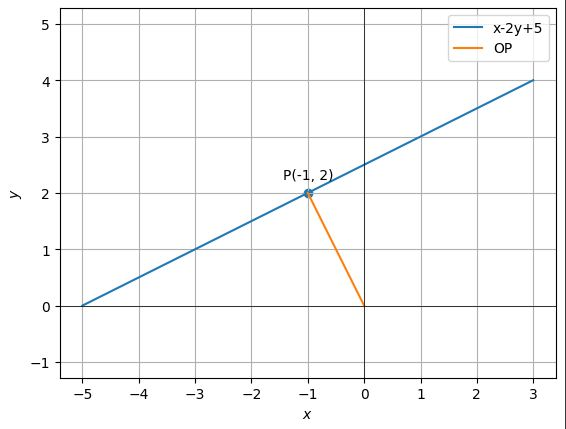
\includegraphics[width=\columnwidth]{figs/graph.jpg}
 % \caption{Graph}
 % \label{fig:pic}
%\end{figure}
%\end{document}
